\documentclass{ltxdockit}
\usepackage{btxdockit}

\usepackage[T1]{fontenc}	
\usepackage[utf8]{inputenc}		
\usepackage[english]{babel}
\usepackage[bitstream-charter]{mathdesign}
\usepackage{tikzducks}
\usepackage{xspace}
\usepackage[most]{tcolorbox}

\KOMAoptions{numbers=noenddot}
\addtokomafont{title}{\sffamily}
\addtokomafont{paragraph}{\spotcolor}
\addtokomafont{section}{\spotcolor}
\addtokomafont{subsection}{\spotcolor}
\addtokomafont{subsubsection}{\spotcolor}
\addtokomafont{descriptionlabel}{\spotcolor}
\setkomafont{caption}{\bfseries\sffamily\spotcolor}
\setkomafont{captionlabel}{\bfseries\sffamily\spotcolor}

\makeatletter
\patchcmd{\paragraph}
  {3.25ex \@plus1ex \@minus.2ex}{-3.25ex\@plus -1ex \@minus -.2ex}{}{}
\patchcmd{\paragraph}{-1em}{1.5ex \@plus .2ex}{}{}
\makeatother

\title{The tikzducks package}
\subtitle{using ducks in tikz}
\author{samcarter}
 
\newcommand{\tikzducks}{\texttt{tikzducks}\xspace}
\definecolor{duckblue}{rgb}{0.0,0.2,0.4}
\lstloadlanguages{[LaTeX]Tex} 

\tcbset{%
	colframe=duckblue,
	arc=2mm,
	fonttitle=\bfseries,
	sidebyside,
	listing options={language={[latex]TeX}, tabsize=2,breaklines},	righthand width=6.5cm
}

\begin{document}

\begin{center}
	{\LARGE \textbf{The \texttt{tikzducks} Package (version 0.2)}}
	
	\large using ducks in \texttt{tikz}
	
	samcarter (alias 
	
\begin{tikzpicture}[scale=0.3,baseline=5pt]
		\duck[body=yellow!50!brown!50!white, 
					longhair=red!50!brown, 
					jacket=blue!50!black]
	\end{tikzpicture}%
	)
	
	\url{https://github.com/samcarter8/tikzducks}

	\today
\end{center}

\section{Introduction}
\label{intro}

The \tikzducks package is a latex package for ducks to be used in \texttt{tikz} pictures. This project is a continuation of an answer at TeX.Stackexchange (\url{https://tex.stackexchange.com/a/347458/36296}).

This package is work in progress (and will probably never be really finished as there is an infinite amount of things which could be added), therefore I would be happy to hear your feedback and ideas how to improve the package. The source code can be found on \url{https://github.com/samcarter8/tikzducks}, including a bug tracker, please make constructive use of it!

\subsection{License}

Copyright \textcopyright\ \texttt{samcarter}. Permission is granted to copy, distribute and\slash or modify this software under the terms of the LaTeX project public licence, version 1.3c \url{http://www.latex-project.org/lppl.txt}.

The shown example ducks are purely fictional characters, any resemblance to real persons is purely coincidental and no copyright infringement is intended.

\subsection{Acknowledgements}

I would like to thank a few fellow user from \href{https://tex.stackexchange.com/}{TeX.Stackexchange}: \href{https://tex.stackexchange.com/users/101651/carlatex}{CarLaTeX} for pointing out the overwhelming need of having a \tikzducks package,
\href{https://tex.stackexchange.com/users/3094/paulo-cereda}{Paulo Cereda} for his contagious enthusiasm for ducks (\emph{Quack!}),
\href{https://tex.stackexchange.com/users/4427/egreg}{egreg} for his help to implement the \texttt{\tikzset{}} interface which makes it much easier to adjust the properties of the ducks to fit the user needs, \href{https://tex.stackexchange.com/users/51022/symbol-1}{Symbol 1} for his help with default key values and last but not least \href{https://tex.stackexchange.com/users/5763/martin-schr%c3%b6der}{Martin Schr\"oder} for his feedback to the code review.

\bigskip\noindent
Without them, this package would not exist!

\newpage
\section{Usage}

The basic usage is fairly simple, to draw a duck:
\begin{tcblisting}{title={basic duck}}

\begin{tikzpicture}
	\duck
\end{tikzpicture}
\end{tcblisting}

To customise this basic duck, the package uses \texttt{pgf} keys. For almost all parts the colour can be changed using \verb|<shape name>=<colour name>|. For example to change the colour of the duck:
\begin{tcblisting}{title={blue duck}}
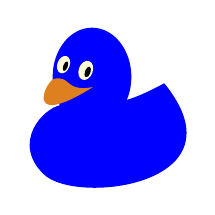
\begin{tikzpicture}
	\duck[body=blue]
\end{tikzpicture}
\end{tcblisting}

If the size of the ducks should be changed:
\begin{tcblisting}{title={scaled duck},	righthand width=3cm}
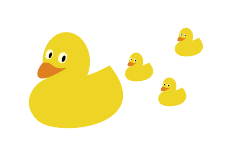
\begin{tikzpicture}[scale=0.6]
	\duck
	\begin{scope}[xshift=90pt, scale=.3, yshift=150pt]
		\duck
	\end{scope}
	\begin{scope}[xshift=60pt, scale=.3, yshift=100pt]
		\duck
	\end{scope}
	\begin{scope}[xshift=80pt, scale=.3, yshift=50pt]
		\duck
	\end{scope}		
\end{tikzpicture}
\end{tcblisting}

\subsection{Body parts}

The various parts of the duck body can also be coloured independently, i.e. \texttt{body}, \texttt{head} and \texttt{bill}:
\begin{tcblisting}{title={harlequin duck}}
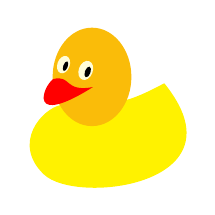
\begin{tikzpicture}
	\duck[body=yellow,
		head=yellow!50!orange, 
		bill=red]
\end{tikzpicture}
\end{tcblisting}

Furthermore using the keyword \texttt{grumpy} the shape of the bill can be changed:
\begin{tcblisting}{title={grumpy duck}}

\begin{tikzpicture}
	\duck[grumpy]
\end{tikzpicture}
\end{tcblisting}

\subsection{Hair styles}

Some duck also like to have nice hair cuts, several different hair styles are available:
\begin{tcblisting}{title={hairy duck}}

\begin{tikzpicture}
	\duck[longhair]
\end{tikzpicture}

\begin{tikzpicture}
	\duck[shorthair]
\end{tikzpicture}


\begin{tikzpicture}
	\duck[crazyhair]
\end{tikzpicture}

\begin{tikzpicture}
	\duck[recedinghair]
\end{tikzpicture}
\end{tcblisting}

And of course the colour of each hair styles can be adjusted:
\begin{tcblisting}{title={coloured hair duck}}

\begin{tikzpicture}
	\duck[longhair=teal]
\end{tikzpicture}
\end{tcblisting}

Eyebrows are also part of the package. The colour choice is a bit complicate for them - if a colour is explicitly specified \verb|eyebrow=<colour name>| this colour is of coursed used. But if no colour is given, it falls first back to the hair colour and only if the duck does not have any hairs, the default colour is applied.
\begin{tcblisting}{title={eye brow duck}}

\begin{tikzpicture}
	\duck[eyebrow]
\end{tikzpicture}
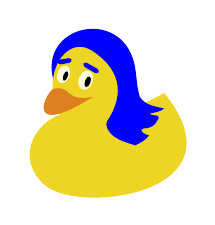
\begin{tikzpicture}
	\duck[longhair=blue, 
		eyebrow]
\end{tikzpicture}

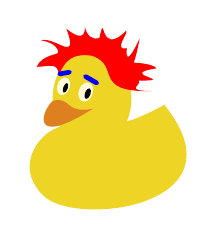
\begin{tikzpicture}
	\duck[crazyhair=red, 
		eyebrow=blue]
\end{tikzpicture}
\end{tcblisting}

\newpage
\subsection{Clothing}

A respectable duck needs a suitable wardrobe. It can choose from a \texttt{tshirt}, a \texttt{jacket} and a \texttt{tie}.
\begin{tcblisting}{title={dressed duck}}
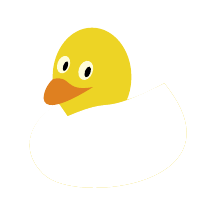
\begin{tikzpicture}
	\duck[tshirt]
\end{tikzpicture}
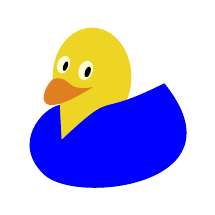
\begin{tikzpicture}
	\duck[jacket]
\end{tikzpicture}

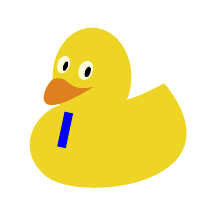
\begin{tikzpicture}
	\duck[tie]
\end{tikzpicture}
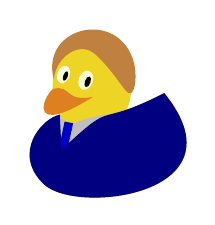
\begin{tikzpicture}
	\duck[tshirt=lightgray, 
			jacket=blue!50!black, 
			tie=blue!80!black, 
			shorthair]
\end{tikzpicture}
\end{tcblisting}

\subsection{Accessoire}

There is a multitude of things a duck might need. All these examples also work without specifying a colour, but giving both examples with and without explicit colour just makes this overview unnecessary long.

\begin{tcblisting}{title={swimming duck}}

\begin{tikzpicture}
	\duck[water=cyan!50!blue]
\end{tikzpicture}
\end{tcblisting}

\begin{tcblisting}{title={alien duck}}
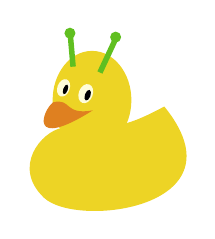
\begin{tikzpicture}
	\duck[alien=green!50!brown]
\end{tikzpicture}
\end{tcblisting}

\begin{tcblisting}{title={hat duck}}

\begin{tikzpicture}
	\duck[hat=red!50!black]
\end{tikzpicture}
\end{tcblisting}

\begin{tcblisting}{title={unicorn duck}}
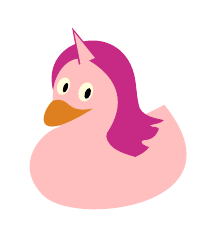
\begin{tikzpicture}
	\duck[body=pink,
	unicorn=magenta!60!violet,
	longhair=magenta!60!violet]
\end{tikzpicture}
\end{tcblisting}

\begin{tcblisting}{title={glasses duck}}
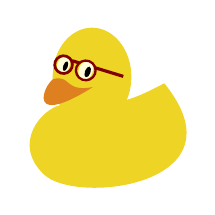
\begin{tikzpicture}
	\duck[glasses=red!50!black]
\end{tikzpicture}
\end{tcblisting}

\begin{tcblisting}{title={sunglasses duck}}

\begin{tikzpicture}
	\duck[sunglasses]
\end{tikzpicture}
\end{tcblisting}

\begin{tcblisting}{title={book duck}}

\begin{tikzpicture}
	\duck[book=\scalebox{0.5}{\TeX}]
\end{tikzpicture}

\begin{tikzpicture}
\duck[book=\scalebox{0.6}{$\pi$}, bookcolour=blue!50!black]
\end{tikzpicture}
\end{tcblisting}

\begin{tcblisting}{title={magic duck}}
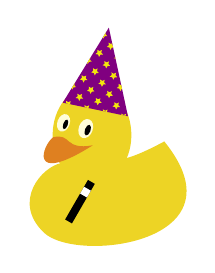
\begin{tikzpicture}
	\duck[magichat,
				magicwand]
\end{tikzpicture}

\begin{tikzpicture}
	\duck[magichat=teal,
				magicstars=cyan,
				magicwand]
\end{tikzpicture}
\end{tcblisting}

\begin{tcblisting}{title={icecream duck}}

\begin{tikzpicture}
	\duck[icecream]
\end{tikzpicture}

\begin{tikzpicture}
	\duck[icecream=brown, flavoura=brown, flavourb=white, flavourc=red]
\end{tikzpicture}
\end{tcblisting}

\section{Further customisation}

This package will never be able to do everything every potential user might want to do, as this number quickly approaches $\rightarrow \infty$. But as the ducks are simply things inside \texttt{tikzpicture}s, all the heavy weapons of the \texttt{tikz} package are available for further customisation.

\begin{tcblisting}{title={adding things to the duck}}
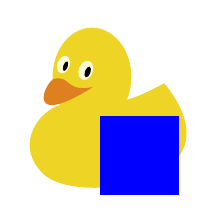
\begin{tikzpicture}
\duck
\path[fill=blue] (2,0) rectangle (1,1);
\end{tikzpicture}
\end{tcblisting}


\begin{tcblisting}{title={monochrome duck}}
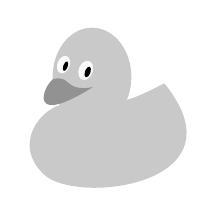
\begin{tikzpicture}
\selectcolormodel{gray}
\duck
\end{tikzpicture}
\end{tcblisting}

\section{Examples}

Some examples how the \tikzducks can be customised:
\begin{tcblisting}{title={samcarter duck},	righthand width=3cm}
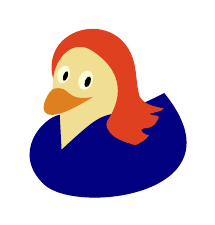
\begin{tikzpicture}
	\duck[body=yellow!50!brown!50!white, 
		longhair=red!50!brown, 
		jacket=blue!50!black]
\end{tikzpicture}
\end{tcblisting}

\begin{tcblisting}{title={Brazil duck},	righthand width=3cm}
\begin{tikzpicture}
\definecolor{brazilgreen}{RGB}{0,155,58}
\definecolor{brazilyellow}{RGB}{254,223,0}
\definecolor{brazilblue}{RGB}{0,39,118}
	\duck[body=brazilyellow,
				shorthair=brazilgreen]
	\path[preaction={fill, brazilblue},pattern=fivepointed stars, pattern color=white] 
		(0.500,1.145) .. controls (0.267, 1.102) and (-0.125,0.657) .. 
		(0.289,0.261) .. controls (0.704,-0.135) and ( 2.863,0.130) .. 
		(1.818,1.419) .. controls (0.938, 0.946) and ( 1.240,1.378) .. 
		(0.513,0.700) -- cycle;
\end{tikzpicture}
\end{tcblisting}

\begin{tcblisting}{title={duck in black},	righthand width=3cm}

\begin{tikzpicture}
	\duck[grumpy, body=yellow!50!brown!50!white, tshirt=white, jacket=black, tie=black, hat=black, sunglasses=black]
\end{tikzpicture}
\end{tcblisting}

\begin{tcblisting}{title={Prof. van Duck}, righthand width=3cm}

\begin{tikzpicture}
	\duck[body=yellow!50!brown!40!white,
		crazyhair=gray!50!white,
		eyebrow,
		glasses=brown!70!black,
		book=\scalebox{0.2}{$E=mc^2$},
		bookcolour=red!20!brown]
\end{tikzpicture}
\end{tcblisting}

\begin{tcblisting}{title={DEK},	righthand width=3cm}
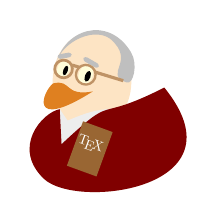
\begin{tikzpicture}
	\duck[body=yellow!50!red!20!white,
		recedinghair=gray!50!white,
		eyebrow,
		tshirt=white!93!black,
		jacket=red!50!black,
		glasses=brown!70!lightgray,
		book=\scalebox{0.5}{\TeX},
		bookcolour=black!20!brown]
\end{tikzpicture}
\end{tcblisting}

\end{document}